\chapter{Design Evaluation Experiment}
\label{chap:de_exp}

\section{Introduction}

The final experiment combines the lessons of the previous experiment to investigate the use of the Rapidly Reconfigurable Research Cockpit (R3C) in a design evaluation study.
The goal of this experiment is to determine if the R3C system can be used in the place of a more traditional evaluation tool.
As previous chapters have discussed, there are a number of self-evident advantages to using the R3C system.
However, there remain some technical limitations to the technology that could hinder adoption.
We found that a button targeting task took more time in our virtual environment than in the real world (Chapter \ref{chap:pointing}).
The following experiment (Chapter \ref{chap:ph_exp}) found that a Fitts' Law task produced a higher throughput using a passive haptics layer, mitigating some of the time increase of targeting buttons in a virtual environment.
In the experiment described in this chapter, we used the R3C system as the simulation tool for a design evaluation study of a cockpit instrument.
The purpose in undergoing this evaluation study is to understand if these limitations would interfere with the metrics that might be used in evaluating a new cockpit design.

We designed an experiment which asks for feedback from subjects who take the role of design evaluators for a cockpit instrument.
The subjects were divided into two groups: one group used an R3C setup to operate the instrument, while the other used a more traditional setup: a touchscreen simulator of the instrument.
This separation of groups will allow a comparison of the feedback from subjects between groups.
Both groups evaluated the same two instrument designs, and subjects were asked to provide feedback using the same questionnaires.
We hypothesize that the R3C system could be used in place of a traditional simulator if the two groups provide similar responses to the designs.
Additionally, we utilized common quantitative metrics to evaluate performance to determine if the conclusions that would be drawn from these change between groups.

\subsection{Background}

\subsubsection{Virtual Prototyping}

Recent advancements in virtual reality technology has renewed interest in the benefits of virtual prototyping, and its use has been increasing across industries - manufacturing \citep{choi_virtual_2015}, assembly \citep{pontonnier_designing_2014}, automotive \citep{bordegoni_mixed_2012,lawson_future_2016}, and medicine \citep{nagendran_virtual_2013}.
The use of virtual environments in design processes is well established.
\citet{aromaa_suitability_2016} reviewed the use of virtual prototypes for human factors/ergonomics (HFE) evaluation.
They found that the fidelity of a VP may not affect subjective results, but that task performance can be affected, hindering the utility of the evaluation itself.
\citet{lawson_future_2016} provided recommendations for incorporating VP in the automotive industry for HFE evaluation, including using haptic feedback and marker-less body tracking.
They found that the use of markers can encumber the participant, affecting evaluation results.

Flight simulation was one of the first applications of virtual environments, and the use of virtual environments for training and development of new cockpits has persisted throughout the years \citep{hancock_human_2008}.
Recent work has investigated augmented reality for cockpit design \citep{wan_mrstudio:_2011}.
The use of virtual reality head-mounted displays have also been studied \citep{yavrucuk_low_2011,aslandere_virtual_2015}.
They did not use any haptic feedback and users interacted with the instruments using hand tracked gloves.
We add to this work with both a unique technical approach and the comparison of performance between a virtual reality design evaluation and a more traditional approach.

\subsubsection{Workload}

Workload is a term that describes the \emph{amount of work} an individual has to do to accomplish a task.
It can refer to the actual amount of work, but typically in the context of aviation and spaceflight it refers to the pilot's perception of the workload.
\citet{hart_development_1988} describes workload as a ``construct that represents the cost incurred by a human operator to achieve a particular level of performance''.
Workload is an important measure for cockpit design as a higher workload can lead to degraded performance or increased errors.
An important factor in the design of cockpit instruments is to reduce the amount of workload.
The workload is measured in this experiment using the NASA Task Load Index (NASA TLX) survey \citep{hart_development_1988}.
The TLX survey asks for a rating of the perceived workload on a number of subscales: Mental Demand, Physical Demand, Temporal Demand, Performance, Effort, and Frustration.
The NASA TLX survey has been widely adopted as a standard for measuring workload \citep{hart_nasa-task_2006}.

\section{Methods}

\subsection{Simulator Setup}

The simulator workstation as configured for each group is shown and annotated in Figure \ref{fig:de_simgroups}.
It was designed to have as much as possible to be the same between the two configurations.
The joystick and instrument were positioned in the same location for each group.
Neither group had out the window visuals, relying only on the attitude indicator on the instrument.
For the Virtual Reality (VR) group, the visuals showed a plain interior of a cockpit, but the out-the-window view was black.
Both groups had an aural indication (a click noise of a button being pressed) when a button was activated on the instrument, using the speakers mounted behind the instrument panel.

\begin{figure}
    \centering
    \begin{subfigure}[t]{0.49\linewidth}
        \centering
        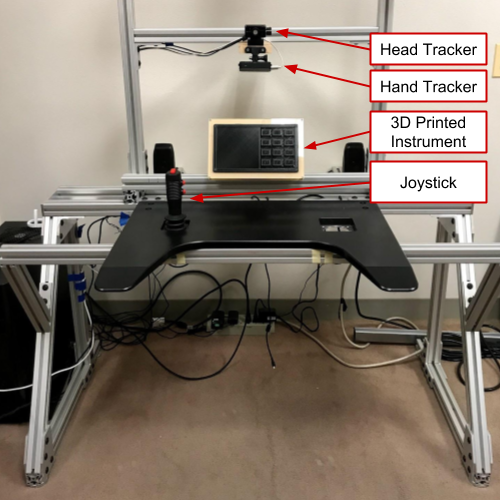
\includegraphics[width=\linewidth]{de_vr_photo.png}
        \caption{VR.}
        \label{fig:de_simgroups:vr}
    \end{subfigure}
    \begin{subfigure}[t]{0.49\linewidth}
        \centering
        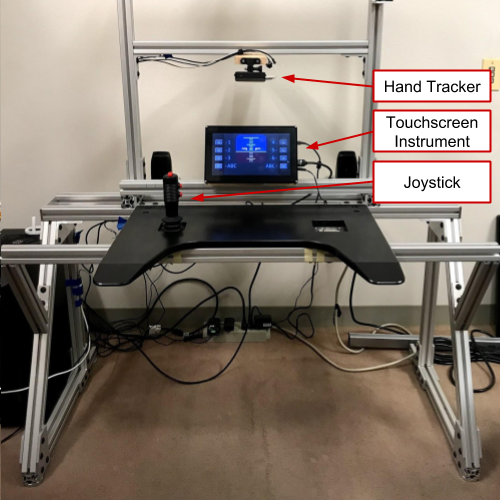
\includegraphics[width=\linewidth]{de_ts_photo.png}
        \caption{TS.}
        \label{fig:de_simgroups:ts}
    \end{subfigure}
    \caption{Simulator Workstation}
    \label{fig:de_simgroups}
\end{figure}

Beyond the VR group using a virtual reality headset for the visuals, the main difference between the two groups was the method for pressing the buttons on the instruments.
The VR group used the hand tracker activated system previously described in Chapter \ref{chap:prototype}.
For this experiment, the buttons were configured to highlight a blue color when the hand tracker registered a finger within the zone.
The zones were extended 0.1in around the border of the button, raised a height of 0.5in above the surface of the button.
When the button was activated after the 150 millisecond delay, the highlight would disappear and the button in the virtual world would move inwards as if it were being pushed in\footnote{Of course, the physical button could not and did not move.}, the press sound would play, and the behavior on the instrument associated with pressing that button would occur.
A separate release sound would play when the finger left the zone after a successful press, and for the VR group the button would move back to its starting position.

The Touchscreen (TS) group used a 10.1 inch capacitive touch screen with resolution of 1024x600.
The active area of the screen was 8.8in by 5.1in, with outside dimensions of 10.4in by 6.7in.
The two instruments were rendered in a web browser using standard HTML elements.
Javascript press and release events were used to simulate the same behavior as described for the VR group, except for the highlighting before a button press.
The visuals of the tracker were rendered on top of the browser window with the same OpenGL rendering code used for the VR group.

%Waveshare 11280

\subsection{Task Design}

Based on the technology available for the simulator base, a number of requirements were laid out that would guide the design of an appropriate task and instrument designs.
The instrument and task required:

\begin{itemize}
    \item Flight task using a standard joystick
    \item Additional task that requires use of multiple buttons on the instrument
    \item Able to develop simulator for both touchscreen and R3C setup %\tinytodo{could explain what this limits}
    \item Able to design two different layouts with one design having distinct flaws
    \item Simple design, yet complex enough task to have sufficient workload
    \item Operationally relevant tasks analogous to those required in a cockpit
\end{itemize}

Ultimately, we designed a task that required number and letter inputs using the buttons, while simultaneously flying a pitch disturbance profile.

\subsubsection{Tracking Task}
\label{sec:de_fdm}

The tracking task display was a standard attitude indicator display, shown in Figure \ref{fig:de_ai_display}.
Each tick corresponds to 1 degree in the dynamics simulation, with major ticks at intervals of 5 degrees.
The attitude indicator was rendered to the size of 3.4 inches square on the instrument.
Subjects controlled the one-dimensional (pitch only) task using a joystick with their left hand.
The joystick is pictured in Figure \ref{fig:de_simgroups}.

\begin{figure}
    \centering
    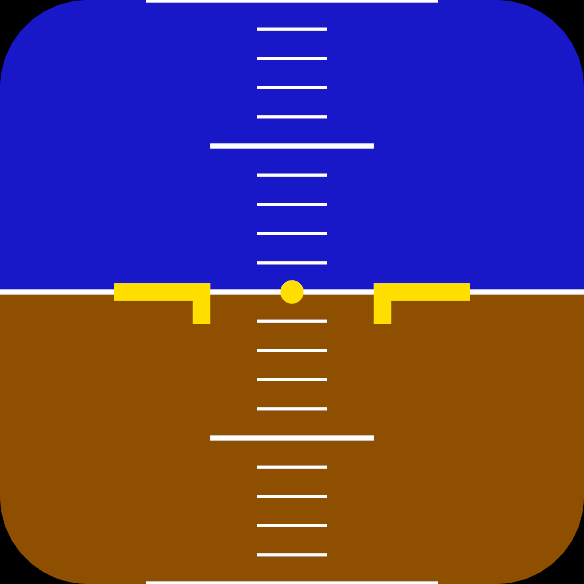
\includegraphics[width=3.4in]{ai_display.png}
    \caption{Attitude Indicator Display}
    \label{fig:de_ai_display}
\end{figure}

The flight dynamics model of the simulator was a stability derivative based model for a Boeing 747 in low altitude flight.
The block diagram of the dynamics is shown in Figure \ref{fig:de_block_diagram}.
The dynamics model was updated and recorded at a rate of 125Hz.
The output of the joystick, $r_{js}$, varies from $-1.0$ to $1.0$, and the gain of $10^{\circ}$ was chosen to ensure the pilot had enough control authority to complete the task.
The flight condition is listed as ``Flight Condition 2'' in NASA CR-2144 \citep{heffley_aircraft_1972}.
This dynamics model was chosen due to availability.
The specifics of the dynamical model were not important other than providing a response similar to an aircraft in flight.
The model was linearized from sea-level flight at an airspeed of 335 ft/s.
The configuration of the airplane had the gear up, no flaps, total weight of 654,000 lbs, and an angle of attack of 7.3$^{\circ}$.
The transfer function of the aircraft dynamics is given as:

\begin{figure}
    \centering
    \centering
    \tikzstyle{block} = [draw, rectangle, minimum height=3em, minimum width=6em]
    \tikzstyle{smallblock} = [draw, rectangle, minimum height=3em, minimum width=3em]
    \tikzstyle{sum} = [draw, circle, node distance=1cm]
    \tikzstyle{input} = [coordinate]
    \tikzstyle{output} = [coordinate]
    \begin{tikzpicture}[auto, node distance=2cm,>=latex']
        \ssp
        \node[input, name=input] {};
        \node[smallblock, right=of input] (K) {$10$};
        \node[sum, right=of K] (sum) {};
        \node[block, node distance=1.5cm, above=of sum] (disturbance) {Disturbance};
        \node[block, right=of sum, text width=5em, align=center] (aircraft) {Aircraft Dynamics};
        \node [output, right=of aircraft] (output) {};

        \draw [draw,->] (input) -- node {$r_{js}$} (K);
        \draw [->] (K) -- (sum);
        \draw [->] (disturbance) -- node {$\theta_D$} (sum);
        \draw [->] (sum) -- node {$\theta_{el}$} (aircraft);
        \draw [->] (aircraft) -- node {$\theta$} (output);
    \end{tikzpicture}
    \medskip
    \caption{Tracking Task Dynamics Block Diagram}
    \label{fig:de_block_diagram}
\end{figure}

\begin{align}
    \mathclap{ % This ignores align for this equation
        \frac{\theta}{\theta_{el}}
        =
        \frac{
            -0.572 (s+0.553) (s+0.0396)
        }{
            (s^2 + 2\zeta_1 \omega_1 + {\omega_1}^2)
            (s^2 + 2\zeta_2 \omega_2 + {\omega_2}^2)
        }
    }\\
    \omega_1 &= 0.0578 & \zeta_1 &= 0.0160 \nonumber \\
    \omega_2 &= 1.12 & \zeta_2 &= 0.798 \nonumber
\end{align}

The disturbance model is based off the model developed in \citet{sweet_identification_1999}.
It is designed to provide a broad spectrum of frequencies for human pilot frequency response identifications \citep{mcruer_mathematical_1974}.
The disturbance is a sum of sines described by:

\begin{align}
    \theta_D = K\sum\limits_{i=1}^{12} \left[ a_i \left(\frac{2\pi k_i}{240} \right) \sin\left( \frac{2\pi k_i}{240}t + \phi_i \right) \right]
\end{align}

The $k_i$ terms are given as,
\begin{align*}
    k_1 &= 7, & k_2 &= 11, & k_3 &= 16 \\
    k_4 &= 25, & k_5 &= 38, & k_6 &= 61 \\
    k_7 &= 103, & k_8 &= 131, & k_9 &= 151 \\
    k_{10} &= 181, & k_{11} &= 313, & k_{12} &= 523
\end{align*}
The amplitude terms are $a_i=0.5$ for $i <= 6$ and $a_i=0.05$ otherwise.
The phase terms, $\phi_i$, were randomly selected on the $(-\pi, \pi)$ interval ensuring a uniform distribution.
This random selection was precalculated for each trial, however the order was repeated for each subject so there was no between subject variance in the disturbance signal.
Furthermore, each subject received the same sequence of disturbance signals for each instrument design.
The disturbance amplitude, $K$, was chosen such that the root-mean square (RMS) of the signal was $3.5$ degrees.
The value of the was chosen through pilot studies to ensure the task was challenging but not overwhelming.

\subsubsection{Prompting Task}

The prompting task was designed to be both a realistic task for a cockpit as well as a demanding task when done in addition with the tracking task.
The task developed required the subjects to read and memorize a short string of characters and enter it back using the buttons on the instrument.
To limit the task physically (by number of buttons) and mentally, the characters used were the number 1 through 6 and the letters A through F.
The prompts were 4 characters long and once the subject started entry the prompt would disappear, forcing them to hold it in working memory.
It has been well established that humans are capable of holding about seven digits in working memory \citep{miller_magical_1956,baddeley_working_1992}.

The sequence of the prompts was separated into 10 second ``windows''.
The prompt would appear randomly between 2 and 3 seconds of the start of the window.
From the time of appearance, subjects were given seven seconds until timeout.
When the subject pressed the first button of the prompt, the prompt itself was cleared and asterisk symbols ($*$) were shown in place of the prompt for each button entry by the subject.
If the subject ran out of time, the text in entry area would return to black.
Although subjects were briefed on the timeout and given practice to learn the pace, no warning or indication of time left was shown during the trials.
Whether they completed the prompt within the time limit, or they timed-out, this process was repeated every 10 seconds.
This meant that subjects had at least 3 seconds of time with no prompt.

The prompts themselves were always composed of three numbers followed by a letter or three letters followed by a number.
This structure was decided upon to provide a consistent pattern, yet still utilize both letters and numbers in every prompt.
The prompts were randomly chosen but were not allowed to have repeat numbers or letters. %, and for the prompts with three letters, common words or acronyms were filtered out (e.g.\ ``BAD'', ``FDA'').
The selection of letters or numbers as the first three characters was randomly chosen as well, with an equal weight to each.

\subsection{Instrument Designs}

The two different designs used were developed to be both realistic as a cockpit instrument design that would be under consideration, yet still have one design with flaws that would be found in a design evaluation.
We developed a `Keypad' design with the prompting task button keys on the right side and the tracking task on the left, and an `Edgekey' design with the prompt buttons split on either side of the tracking task display.
The tracking task display was the same size on the display for both designs.
The prompting task text was placed below the tracking task display, and the same font, size and color was used for both designs.
The prompting task text font was approximately 0.62in tall.
These were kept consistent to limit the number of possible variables between the two designs.
The prominent difference is the placement and behavior of the buttons which is described in this section.

The Keypad design is pictured in Figure \ref{fig:de_keypad_design}.
The buttons are 1in by 0.75in, with about 0.26in between buttons horizontally and 0.38in vertically.
Each button has the label directly on the top of the button.
The 3D printed instrument used for the VR group had the buttons raised a height of 0.31in from the surface of the instrument.
The button labels were also raised to provide a tactile feedback.
The font was approximately 0.36in tall, and the labels were embossed above the button surface 0.05in.

\begin{figure}
    \centering
    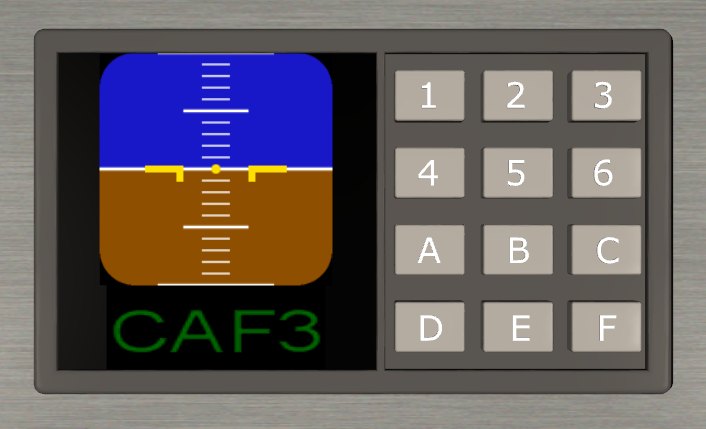
\includegraphics[width=\textwidth]{keypad_vr.png}
    \caption{Keypad Design}
    \label{fig:de_keypad_design}
\end{figure}

\begin{figure}
    \centering
    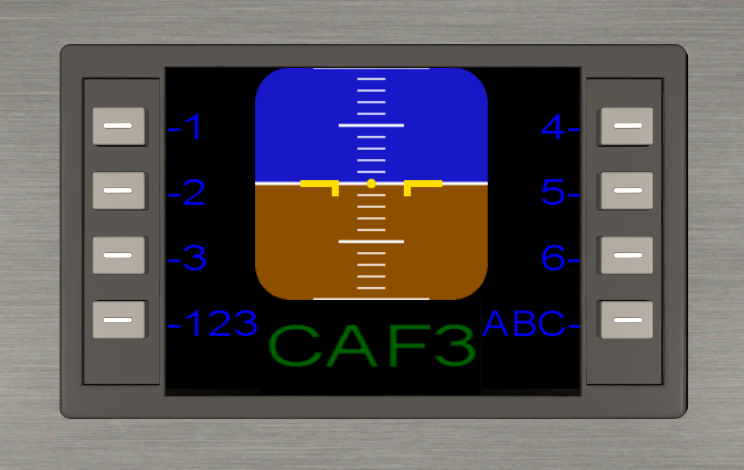
\includegraphics[width=\textwidth]{edgekey_vr.png}
    \caption{Edgekey Design}
    \label{fig:de_edgekey_design}
\end{figure}

The Edgekey design is pictured in Figure \ref{fig:de_edgekey_design}.
In this design, there is not a single button for every number and letter.
Instead, the bottom button on either side would switch the behavior (and labels) of the remaining six buttons from being 1 through 6 to A through F.
In other words, the bottom ``switching'' buttons would change the rest of the buttons from the numbers to the letters, and vice-versa.
The labels were placed offset from the button on the ``screen'' portion of the instrument, allowing them to change dynamically.
The fonts were approximately 0.32in tall, and were blue on the screen.
The buttons are slightly smaller in this design, at 0.76in by 0.55in.
A smaller button size was needed to fit the labels and the buttons side by side.
The spacing between buttons vertically is the same as the Keypad design at 0.38in.
The center to center distance between the two sides of the button rows is 7.3in.
The 3D printed instrument version had raised nubs on each button covering half the width, 0.08in tall and raised 0.05in.
As with the Keypad design, the buttons had the same height of 0.31in from the surface.

While some of the more subtle differences were expected to be noted by the evaluation study (e.g.\ having smaller buttons, different position of the flight task), the major flaw designed into the Edgekey design was the switching key to change from letters to numbers and back.
This additional action fundamentally changed the demands of the task, as the subjects now had to press this additional button to change labels at least once per prompt.
The cognitive workflow of the subject is diagrammed in Figure \ref{fig:de_flowchart}.
The additional mental effort of the Edgekey design is shown in the dashed box, where the subject has to verify the state of the instrument and possibly press the switch button before they press the buttons of the prompt.
Since the prompts were kept as a consistent format of three of the same type and fourth of the other, this extra work was easily skipped for most buttons, and anticipated between the third and fourth button.
There was no guarantee that the next prompt would start with the instrument in the correct state for the new prompt, so there was always an additional cognitive load in determining whether a switch was necessary at the beginning of the prompting window, which would be accompanied with the physical effort if the switch was needed.

\begin{figure}
    \centering
    \tikzstyle{decision} = [diamond, draw, fill=blue!20, text width=7em, text badly centered, inner sep=0pt]
    \tikzstyle{block} = [rectangle, draw, fill=blue!20, text width=8em, text centered, rounded corners, minimum height=2em]
    \tikzstyle{line} = [draw, -latex']
    \tikzstyle{cloud} = [draw, ellipse,fill=red!20, minimum height=2em]
    \begin{tikzpicture}[auto]
        \node [block] (read) {Read Prompt};
        \node [block, below=of read] (memorize) {Memorize Prompt};
        \node [block, below=of memorize] (recall) {Recall $n^{\mathrm{th}}$ Character};

        \node [decision, below=of recall] (design) {Design?};
        %\node [cloud, below=of recall] (Keypad) {Keypad};

        \node [draw=none, text width=7em, below=2cm of design] (targetjoin) {};
        \node [block, below=1cm of targetjoin] (target) {Find \& Target $n^{\mathrm{th}}$ Button};
        \node [block, below=of target] (press) {Press $n^{\mathrm{th}}$ Button};
        %\node [draw=none, left=of target] (nloop1) {};
        \node [draw=none, below=0.5cm of design] (keypadlabel) {Keypad};
        \node [draw=none, left=of keypadlabel, text width=6em, text centered] (nloop) {Repeat for 4 Characters};

        \node [decision, right=1.5cm of targetjoin] (decide) {Are labels for $n^{\mathrm{th}}$ character shown?};
        %\node [cloud] (Edgekey) at (design -| decide) {Edgekey};
        \node [block, below=of decide] (targetswitch) {Find \& Target Switching Button};
        \node [block, below=of targetswitch] (pressswitch) {Press Switching Button};
        \node [block, below=of pressswitch] (recall2) {Recall $n^{\mathrm{th}}$ Character};

        \path [line] (read) -- (memorize);
        \path [line] (memorize) -- (recall);
        \path [line] (recall) -- (design);
        %\path [line] (design) -- node [fill=white, near start, center] {Keypad} (target);
        \path [line,-] (design) -- (keypadlabel);
        \path [line] (keypadlabel) -- (target);
        \path [line] (target) -- (press);
        \path [line,-] (press) -| (nloop);
        \path [line] (nloop) |- (recall);

        %\path [line, dashed] (recall.south) ++(0,-0.5cm) -| (Edgekey);
        \path [line] (design) -| node [near start, above] {Edgekey} (decide);
        \path [line] (decide) -- node [above] {Yes} (targetjoin.center);
        \path [line] (decide) -- node {No} (targetswitch);
        \path [line] (targetswitch) -- (pressswitch);
        \path [line] (pressswitch) -- (recall2);
        \path [line] (recall2.east) -- ++(1.0cm,0) |- (decide.east);

        \draw[thick, dashed] ($(design.east)+(0.8,1.0)$) rectangle ($(recall2.south east)+(1.6,-0.6)$);
        %\draw[thick, dashed] ($(decide.north west)+(-1.8,3.3)$) rectangle ($(recall2.south east)+(1.3,-0.6)$);

    \end{tikzpicture}
    \medskip
    \caption{Prompting Task Flowchart of Cognitive Work for Each Design. Extra work of Edgekey design enclosed in dashed line box.}
    \label{fig:de_flowchart}
\end{figure}

\subsection{Experiment Design}

Subjects were divided into the two groups, Touchscreen (TS) and Virtual Reality (VR).
The overall sequence of the experiment started with a training session on the simulator and the task, followed by an evaluation session for each of the two designs, finishing with questionnaires asking subjects to evaluate the two designs.
The timeline of the experiment was the same for each subject, except for counterbalancing the order that the designs were evaluated.
The training portion started with a slide deck explaining the tasks, the simulator that the subject was using (depending on which group they were in), and the functionality of the two designs they were to evaluate.
Next, they performed practice trials with just the tracking task and then just the prompting task.
The practice trials of the tracking task were 60 seconds long and repeated until the subjects' performance had flat-lined.
This took between three to six trials for each subject.
%After basic familiarity with the technology

\begin{figure}
    \centering
    \begin{subfigure}[t]{0.49\linewidth}
        \centering
        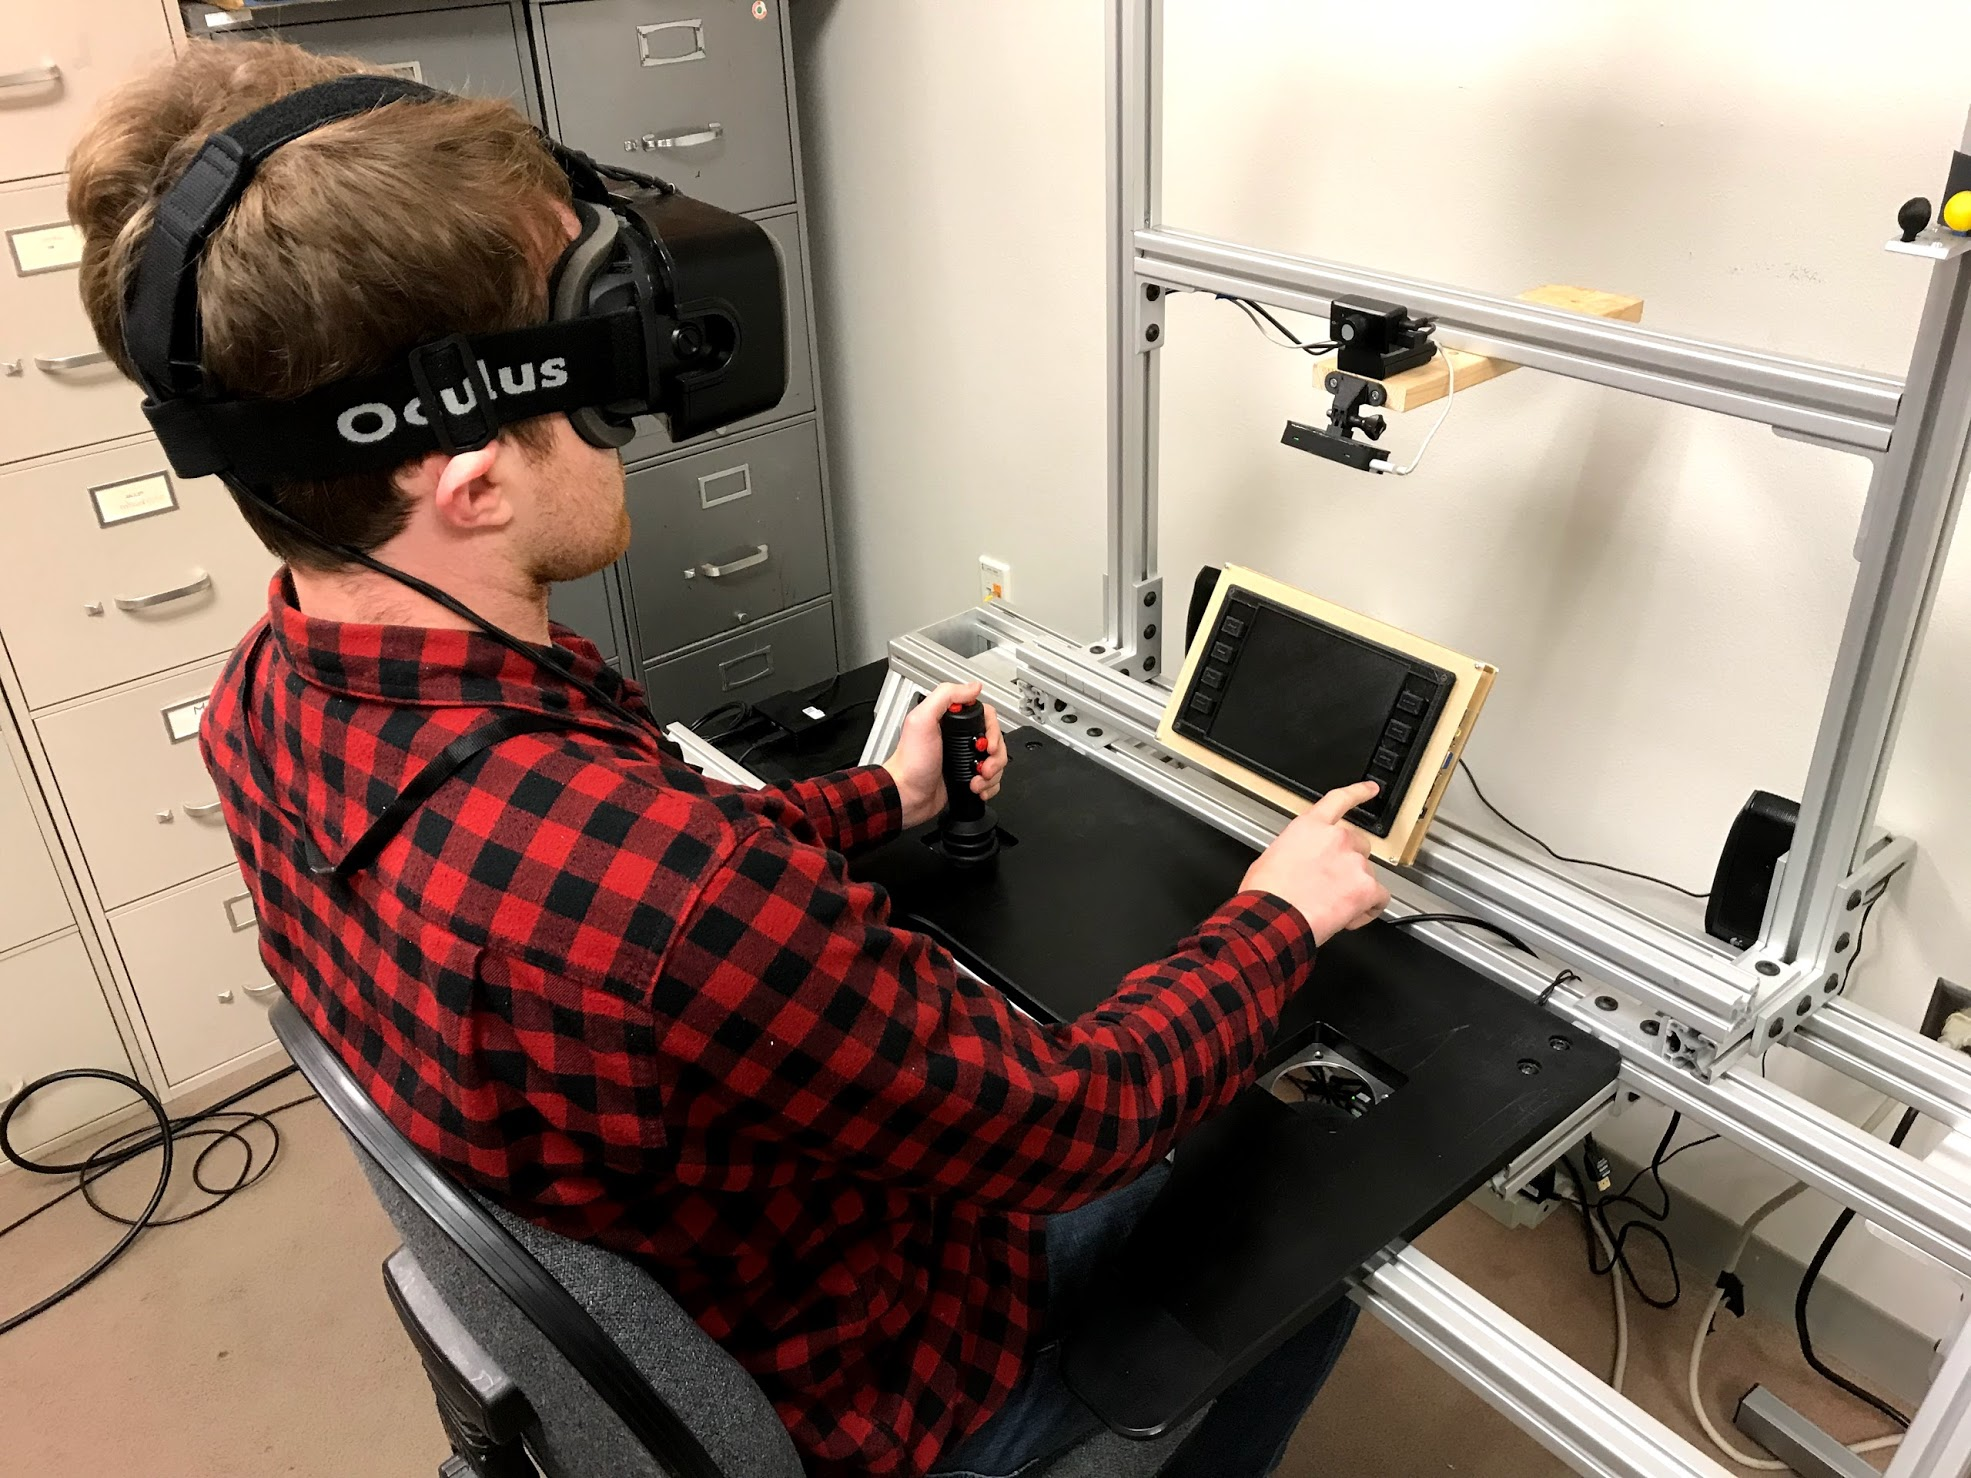
\includegraphics[width=\linewidth]{de_vr_user.jpg}
        \caption{VR.}
        \label{fig:de_userpic:vr}
    \end{subfigure}
    \begin{subfigure}[t]{0.49\linewidth}
        \centering
        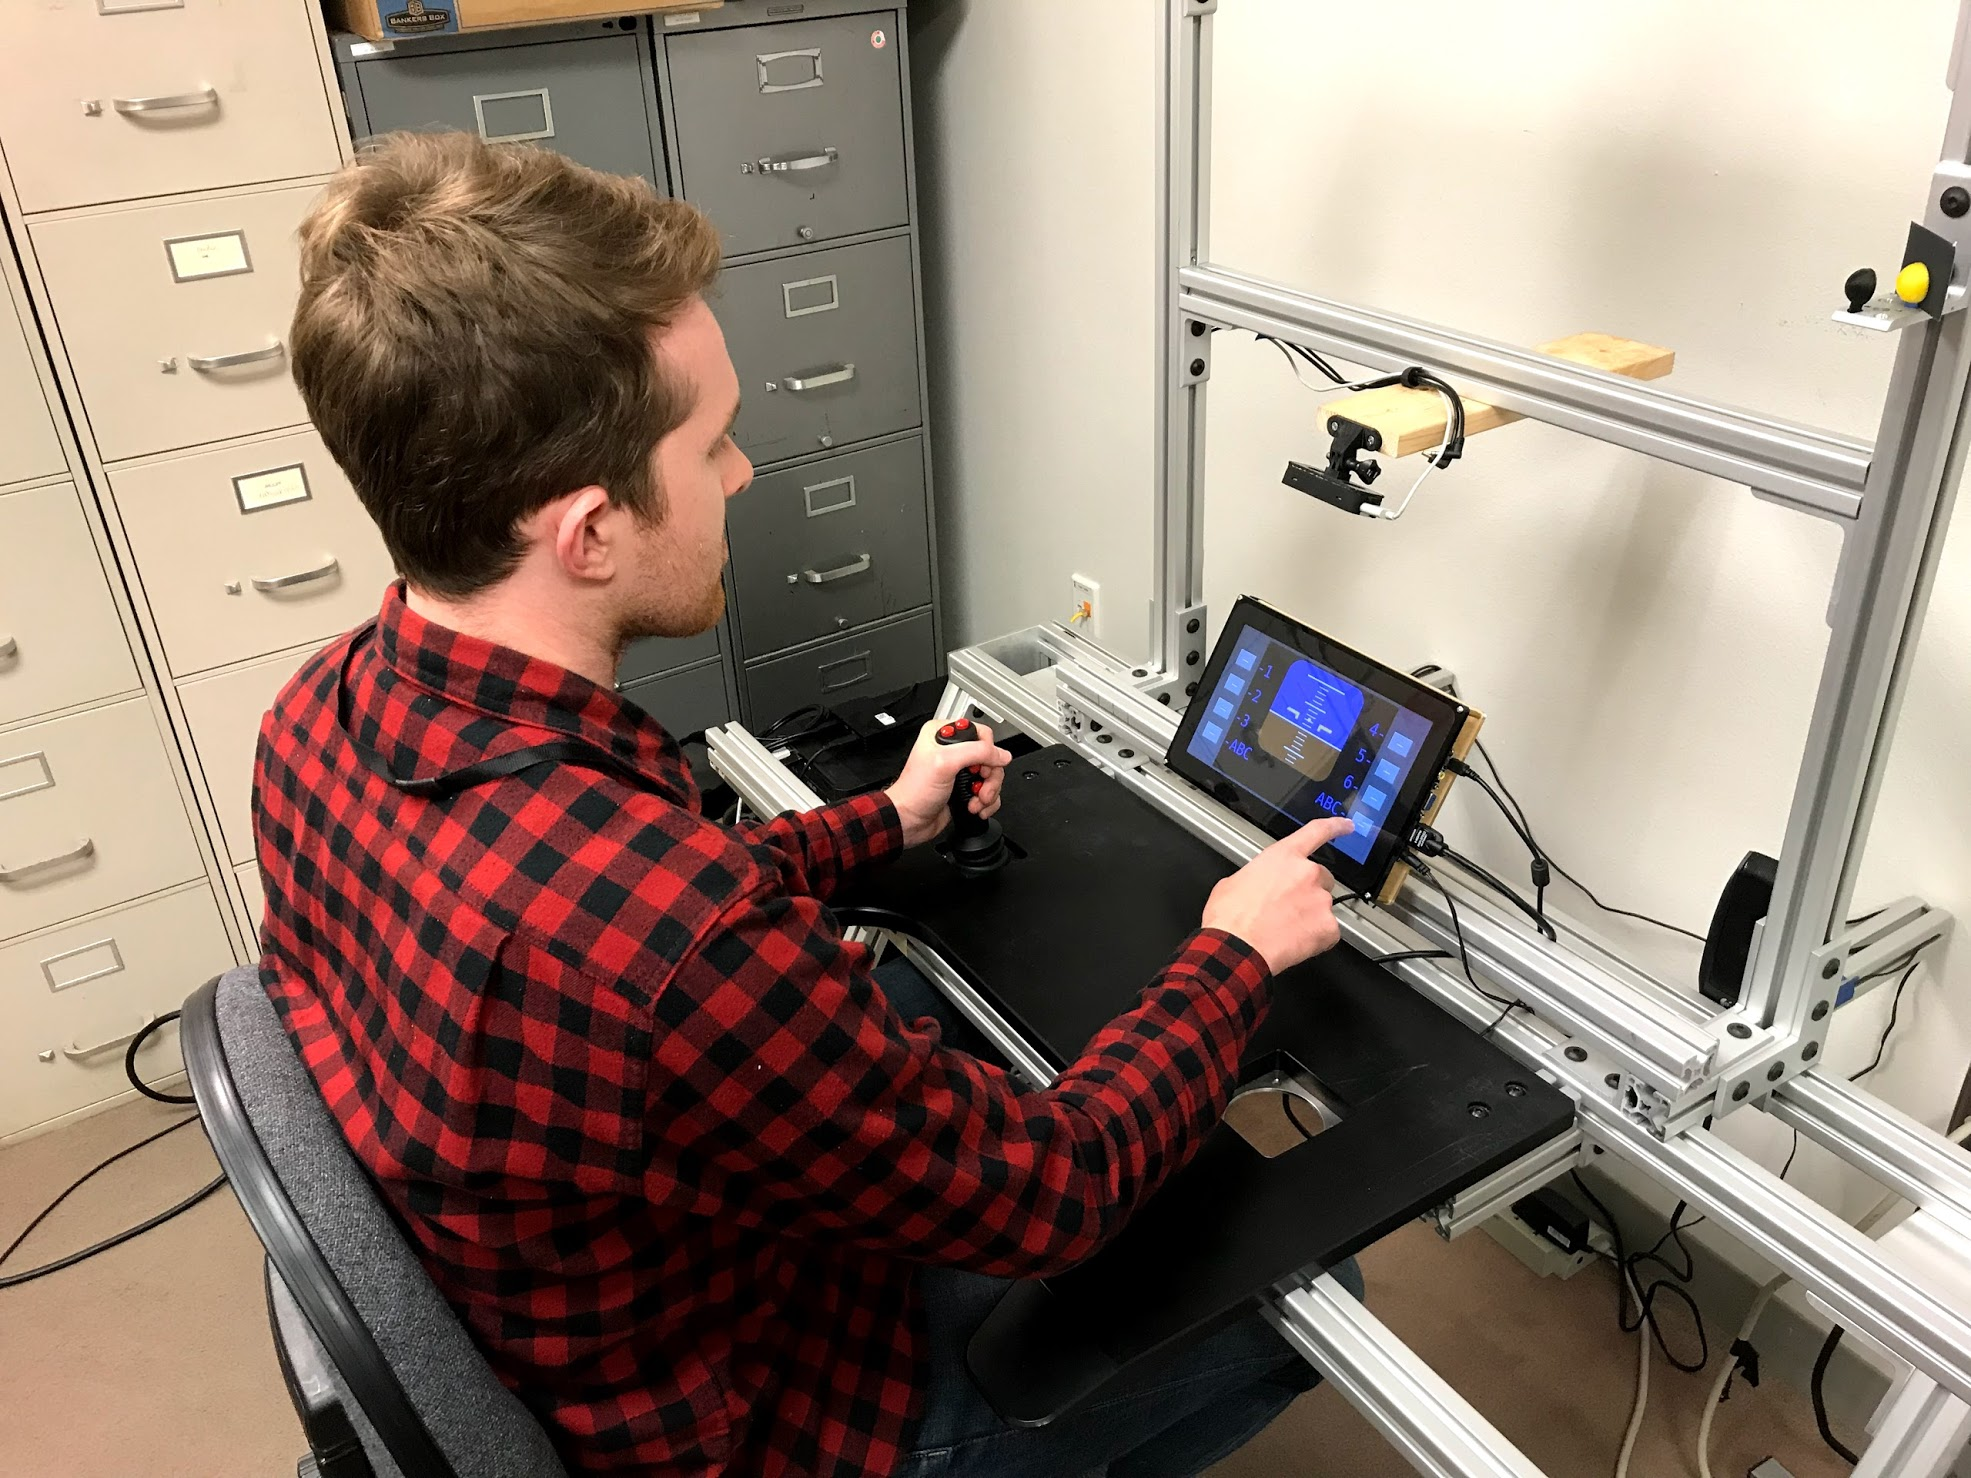
\includegraphics[width=\linewidth]{de_ts_user.jpg}
        \caption{TS.}
        \label{fig:de_userpic:ts}
    \end{subfigure}
    \caption{Simulator Workstation}
    \label{fig:de_userpic}
\end{figure}

For the evaluation sessions with each design, they performed six trials with both tasks.
The first three were a minute long, and were considered practice trials, and not included in the data analysis, though this was not communicated to the subjects.
The following three trials were two minutes each, and were used for the analysis.
Each evaluation session concluded with a two minute trial of just the tracking task without the prompting task.
This was included to investigate if the subject had improved or fatigued at the tracking task throughout the experiment.

The independent variables of the experiment are Group and Design.
The Group is the simulator the subject used, a between subjects factor, and either TS or VR.
The Design is a within subjects factor, the two instrument designs that every subject evaluated --- Edgekey and Keypad.

\subsection{Dependent Measures}
\label{sec:de_dependent}

The dependent measures were chosen to evaluate the performance of each task individually as well as the workload of the subject.
For the tracking task, the root-mean square error (RMSE) was calculated for each trial \citep{harris_human_2011}.
The error in this case is simply the pitch shown to the subject, the output of the flight model described in Section \ref{sec:de_fdm}.

The prompting task has two dependent measures, for speed and accuracy.
For speed we consider the \textit{response time}, defined as the time between when the prompt is first shown to the subject and when they press the first button of their response entry.
The accuracy is measured by how many prompts they complete correctly.
Twelve prompts are shown to the subject within each trial.
The response time was meaned per trial first and then per design for each subject, and the number of correct prompts is meaned per design for each subject.

A NASA Task Load Index (TLX) survey was administered after they completed each design to measure the workload of the subject.
The TLX survey asks for a rating of their workload between 0-100 for the following subscales: Mental Demand, Physical Demand, Temporal Demand, Performance, Effort, and Frustration.
Our implementation allowed selection of the ratings within increments of 5, and included anchors of ``Low'' and ``High'' at the extrema of 0 and 100, respectively (except for Performance, which uses ``Good'' and ``Bad'').
The midpoint was also visually indicated with a larger tick.
The ranked pairs modification was used and completed for both times the subject took the survey.
This modification asks the subject, for each of the pairwise combinations of subscales, which they felt contributed more to their workload.
The number of times they select each subscale is used a weight to calculate a weighted mean for the total TLX score.

Finally, the subjects were given a questionnaire asking for their feedback on each instrument design.
For each design, the subjects were asked the following questions:
\begin{itemize}
    \item Please comment on any difficulties you had performing the prompting task with this design especially in contrast to the other design.
    \item Please comment on anything you liked in this design.
    \item Please comment on anything you did not like in this design.
    \item Any other comments?
\end{itemize}
Additionally, the following questions were asked:
\begin{itemize}
    \item Which instrument design did you prefer? Why?
    \item Did you experience any physical fatigue during the experiment? Where?
    \item Any other comments?
\end{itemize}
An open form text box was used for the response field for each of these questions.

In a standard design evaluation study, the feedback received from the users in this questionnaire (and other debriefing interviews) would often be the main source for carrying out re-design.
The purpose of this feedback in this experiment is to determine and document in which ways does this feedback differ.
For example, if most subjects in one group noted issues with the size of a button, while no one in the other group found an issue with that button, this would indicate that using this VR system may not highlight the same issues regarding button sizes.
The groups were purposely left ambiguous in the example, as it does not matter which group found the flaw and which group did not comment on it.
Although we could postulate as to which group are ``correct'' in their evaluation of the instrument, it is not a useful exercise, as the only result is to document what potential differences could arise so that users of this system can be aware.

With that goal in mind, the analysis of the feedback questions seeks to find differences between the groups.
The sentences from the open form responses were first separated into single feedback comments, and summarized using common language.
If a single subject repeated the same comment in the answers to multiple questions, they were only counted once.
Each of these simplified feedback comments were assigned to a category or overall summary of their feedback.
This process was completed separately for each group.
We aim to look for feedback that is unique to a certain group or feedback that receives a higher frequency of comments in one group.
This will provide a summary of where the groups provide the same feedback and where they provide differing feedback.

\subsection{Hypotheses}

The main hypothesis of this experiment is that the use of a VR/R3C simulator will not affect the conclusions of a design evaluation study, compared to a traditional touchscreen simulator.
We do expect that some of the dependent measures may have a significant difference in Group or a significant difference in Design.
The more important measure for us, however, is the interaction effect.
This will test if the change between Designs is similar for the two Groups.
If this is the case, then it may indicate that an evaluation study using one of these simulators could draw differing conclusions of an evaluation study using the other.
Statistically, we will test the hypothesis that there exists no interaction effect between Group and Design for any of our dependent measures.

Additionally, the two tracking only trials performed at the end of each evaluation session, as well as the final tracking only training trial, will be used to investigate if the subjects were still learning the tracking task.
The concern if subjects became more trained in the tracking task is that it could lower their amount of attention to that portion of the task, causing a change in performance on the prompting task that was not due to the design change.
These hypotheses are enumerated here:

\begin{enumerate}[label={H\arabic*.}]
    \item The tracking task RMSE will have no interaction effect between Group and Design
    \item The prompt response time will have no interaction effect between Group and Design
    \item The number of correct prompts will have no interaction effect between Group and Design
    \item The NASA TLX scores will have no interaction effect between Group and Design
    \item The tracking task RMSE for the last training trial and the tracking only trials will not change throughout the experiment
\end{enumerate}

\subsection{Statistical Tests}

The quantitative dependent measures are tested with a two-way ANOVA, with one within subjects factor (Design) and one between subjects factor (Group).
The Design factor contains two levels, the two designs each subject tested, Edgekey and Keypad.
The Group factor also contains two levels, the VR (Virtual Reality) group and the TS (Touchscreen) group.
When the ANOVA showed significance in the interaction test, post-hoc repeated measured t-tests were undertaken to determine the significance of Design within each Group.
Independent samples t-tests were used to test the significance of Group within each Design.
The last hypothesis testing the effects of learning on the trials with only the tracking task will be tested with a two-way ANOVA, with the Group as a between subjects factor, and the trial number as a within subjects factor.
The trial number is chronological in the order the subjects performed them.
The first trial was the last tracking only training trial, and the next two were tracking only trials at the end of each design evaluation.

Statistical significance level was corrected using the Bonferroni correction considering the 5 hypotheses being tested.
All effects were considered statistically significant at the 0.01 level ($\alpha = 0.05/5 = 0.01$).
Effects which have a significance level between $0.05<p<0.01$ are considered to be marginally significant.

\section{Results}

\subsection{Demographics}

Twenty-three subjects were recruited from the UC Davis engineering undergraduate and graduate student population.
Twelve subjects were placed in the VR group, and the remaining eleven in the TS group.
The mean age was 21.0 ($\sigma = 3.14)$, with 19 male and 4 female subjects.
The genders were balanced between the two groups.
Most subjects had no flight experience (two were student pilots), and all of the VR group subjects indicated that they had less than one hour of experience using virtual reality headsets.
It should be noted that the subjects are not the beneficial population of the research.
The task and experiment was designed with this in mind and mitigated through training and the simplicity of the task design.

\subsection{Performance Measures}

\subsubsection{Tracking Task RMSE}

\begin{figure}
    \centering
    \includegraphics[width=4.0in]{{rmse.4.0x4.0}.png}
    \caption{Factor Plot of RMSE}
    \label{fig:de_factor_rmse}
\end{figure}

The performance of the tracking task was measured using the root-mean square error (RMSE) of the pitch.
The effect of Group yielded an $F$ ratio of $F(1, 21) = 21.4, p < 0.001$ indicating a significant difference between VR ($M=1.28\mathrm{deg}, \sigma=0.38\mathrm{deg}$) and TS ($M=1.97\mathrm{deg}, \sigma=0.38\mathrm{deg}$).
In both groups, subjects were performing the tracking task using the same joystick.
The most direct factor that could contribute to the decreased performance in the tracking task for the VR group is the loss of visual acuity in the tracking task display due to the technical limitations of the VR head-mounted display.
Indirectly, the additional workload of the prompting task could be taking attention away from the tracking task.
The effect of Design indicated a marginally significant difference ($F(1, 21) = 5.94, p=0.024$) for the tracking task RMSE between Keypad ($M=1.57\mathrm{deg}, \sigma=0.51\mathrm{deg}$) and Edgekey ($M=1.70\mathrm{deg}, \sigma=0.52\mathrm{deg}$).
The only change in the tracking task display between the two instrument designs is a small change in position.
It moves from being on the left side for the Keypad to the middle for the Edgekey.
Since there was no change otherwise, this suggests that any difference on the tracking task performance between the designs would be related to additional workload from the prompting task.
The interaction effect was not significant ($F(1, 21) = 0.17, p=0.69$).

We can investigate the trials where the subjects were only doing the tracking task to further investigate the change in performance between the two groups.
The subjects ran a single trial that was just the tracking task without the prompting task at the end of each evaluation session.
These trials were included to be used as a test of the assumption that the subjects were no longer learning, but can also be used as a test of the Group factor on the tracking task performance.
The effect of group on RMSE for the tracking-only trials yielded a marginally significant difference ($F(1, 21) = 4.81, p = 0.039$) between the VR Group ($M=1.32, \sigma=0.50$) and the TS Group ($M=0.91, \sigma=0.43$).
There was no significant difference for the effect of design ($F(1,21) = 0.068, p=0.80$).
The interaction effect between group and design was also not significant ($F(1,21) = 3.21, p=0.087$).

Although the tracking only trials found a marginally significant difference for the group, the difference was much more distinct for the trials with both tasks.
This indicates that when the subjects were focused on the single task, they were able to mitigate most of the visual resolution differences between using a touchscreen and the virtual reality screen.
Additionally, the marginally significant difference between the designs for the trials with both tasks was reduced to no significance when the additional prompting task was removed.
This also points to the additional workload of the prompting task causing a performance drop on the tracking task.
The factors leading to the added workload of the prompting task are investigated in the next performance measures discussed.

\subsubsection{Prompt Response Time}

\begin{figure}
    \centering
    \includegraphics[width=4.0in]{{reaction_time.4.0x4.0}.png}
    \caption{Factor Plot of Response Time}
    \label{fig:de_factor_response}
\end{figure}

The first measure of the prompting task is the response time of the subject.
The response time is defined as the time from the prompt is shown to each subject until they press the first button of the prompt.
For the Edgekey design, it would be possible that the subject had to start with the switching button if the new prompt did not start with the same mode (letters or numbers) as the previous prompt (see Figure \ref{fig:de_flowchart}).
Since this button would not clear the prompt when it was pressed, it is not considered the first button of their entry.
However, this would still require an additional movement of the subject, adding additional time.
For this reason, the prompts which required the subject to start with the switch key are filtered out of this analysis.
After filtering, 885 of the total 1700 prompts recorded for the Edgekey design were kept.

The response time was unique among the dependent measures, as all tests were insignificant.
The effect of group yielded an $F$ ratio of $F(1, 21) = 1.19, p = 0.29$ indicating no significant difference between VR ($M = 2812\mathrm{msec}, \sigma = 383\mathrm{msec}$) and TS ($M = 2594\mathrm{msec}, \sigma = 567\mathrm{msec}$).
One factor that could influence the response time between groups is the additional time to activate a button in the VR environment versus the touchscreen.
The touchscreen subjects were using a familiar interface for activating the buttons, while the VR subjects needed to activate the button with the virtual hand.
However, a large portion of the response time for the subject is their cognitive processing of the prompt -- recognizing the new prompt has appeared, reading it, then memorizing it.
Beyond potential differences in the visual environment, the cognitive portion should not take more time for one group or the other.
A potential reason that there could be a lower than expected difference between the group means is that some VR subjects learned to keep their hand closer to the instrument so that the hand tracker could keep it in view.
When the hand tracker lost view of the hand, the re-acquisition time could be significant, so holding it close to the instrument would prevent this from happening.
This issue comes up again when looking at the subjects' response to questions about fatigue.

The effect of design was also insignificant ($F(1, 21) = 0.68, p = 0.42$) between Keypad ($M=2728\mathrm{msec}, \sigma=512\mathrm{msec}$) and Edgekey ($M=2687, \sigma=471\mathrm{msec}$).
The biggest difference between the two designs is the switching key on the Edgekey design.
As described above, the need for an additional switch press before the first prompt button was filtered out, so we are only comparing prompts where the first button was available right away to the subject.
Even though the physical requirements were filtered out, subjects still need to verify that the labels are in the correct state for starting entry.
Since the Edgekey design had more time pressure due to the need for the switch key, subjects could have learned to respond quicker to adapt for this.
However, these differences in the design did not appear to have a significant effect on the response time.
Finally, the interaction effect was not significant ($F(1, 21) = 0.001, p = 0.96$).

\subsubsection{Prompts Correct}

\begin{figure}
    \centering
    \includegraphics[width=4.0in]{{correct_prompts.4.0x4.0}.png}
    \caption{Factor Plot of Correct Prompts}
    \label{fig:de_factor_correct}
\end{figure}

The second measure of the prompting task is the accuracy of the subjects in correctly completing the prompt.
To get the prompt correct includes two important components for the subject.
First, they must remember the prompt as they enter it, and second, they must be able to physically press the buttons within the seven second response window.
For the statistical test, we are using the count of how many prompts each subject completed successfully per trial.
Among the incorrect prompts, we can differentiate between whether the subject entered the prompt incorrectly (failure to remember the prompt) or whether the subject ran out of time (failure to physically press the buttons).
These counts are reported to help analyze the results, but are not used in the statistical tests.
There were 12 prompts per trial, and every subject completed three trials for each design.

The number of correct prompts had a significant interaction effect between group and design ($F(1, 21) = 27.8, p < 0.001$), meaning the main effects must be interpreted with the post-hoc tests as well.
Both main effects were significant, the effect of group yielded an $F$ ratio of $F(1, 21) = 43.9, p < 0.001$ while the effect of design yielded an $F$ ratio of $F(1, 21) = 64.1, p < 0.001$.

For the effect of design on the VR group, the repeated measured t-test indicated a significant difference ($t(11) = 8.0, p < 0.001$) between the Keypad ($M = 8.11, \sigma = 1.62$) and the Edgekey ($M = 4.00, \sigma = 2.37$)
The TS group had a marginally significant difference ($t(10) = 2.28, p = 0.045$) between Keypad ($M = 10.6, \sigma = 0.96$) and the Edgekey ($M = 9.82, \sigma = 1.38$).
These results indicate that both groups had trouble with the additional time pressure caused by the Edgekey design requiring the use of the switch key.
The TS group performed a lot closer to their performance in the Keypad design, however, only getting approximately 1 fewer prompt correct.
The VR group had much more difficulty in the Edgekey design, correctly completing about half as many as they completed in the Keypad design.
However, they had more difficulty in both designs compared to the TS group.

\begin{figure}
    \centering
    \includegraphics[width=6.0in]{{prompts_stacked.6.0x4.0}.png}
    \caption{Result of prompts}
    \label{fig:de_correct_stacked}
\end{figure}

This agrees with the post-hoc tests for differences between groups within each design.
These tests had significant effects for both the Keypad design ($t(21) = 4.44, p < 0.001$) between the VR group and the TS group, and the Edgekey design ($t(21) = 7.05, p < 0.001$) between the VR group and the TS group.
The main effect of group clearly has a meaningful effect, which found the VR group ($M = 6.05, \sigma = 2.88$) had significantly fewer correct prompts than the TS group ($M = 10.2, \sigma = 1.2$).
This difference is largely due to subjects not being able to complete the prompt.
Figure \ref{fig:de_correct_stacked} shows the breakdown of the mean result of each trial for each group and design.

Across all groups and designs, very few prompts were completed that were incorrect, and most of the difference in number completed correctly is due to the incomplete prompts.
A contributing factor for this would be the method of button activation used for the VR group combined with the time pressure.
Another contribution would be the limitations of the hand tracker.
When the hand tracker lost tracking or gave bad information, it became hard or impossible for the subject to activate a button until the hand tracker returned to normal.
When this happened in the middle of a prompt, the amount of time it took to recover from the bad tracking would lead to a timeout on the prompt entry, causing an incomplete prompt.
The variance of number correct was also much larger in in the VR group, which could be caused by some subjects adapting to the unfamiliar VR environment more rapidly.

\subsubsection{NASA TLX}

\begin{figure}
    \centering
    \includegraphics[width=4.0in]{{tlx.4.0x4.0}.png}
    \caption{Factor Plot of NASA TLX}
    \label{fig:de_factor_tlx}
\end{figure}

After the subject completed their trials for each design, they filled out a NASA TLX workload survey.
Their scores, weighted means by the pairwise comparisons, are used here as a measure of their self-reported workload.
The interaction effect between group and design was found to be significant ($F(1, 21) = 8.25, p < 0.001$).
The main effects showed a significant difference in design ($F(1, 21) = 23.6, p < 0.001$), but not in group ($F(1, 21) = 1.69, p = 0.21$).
This could mean that the group did not affect the TLX score, but in the presence of an interaction effect, the post-hoc tests guide the interpretation.

The repeated measures t-tests indicated significance between designs for the VR group ($t(11) = -4.20, p = 0.001$) between the Keypad design ($M = 54.4, \sigma = 20.4$) and the Edgekey ($M = 85.6, \sigma = 11.2$)
There was a marginally significant difference between designs for the TS group ($t(10) = -2.72, p = 0.02$) between the Keypad design ($M = 61.5, \sigma = 4.46$) and the Edgekey ($M = 69.2, \sigma = 10.1$).
The effect of design was much stronger in the VR group, but both groups indicated respectively higher workload on the TLX scores for the Edgekey design.
This follows from the experimental design which predicted that the Edgekey design would be more difficult.
One factor that could have contributed to a larger difference in scores for the VR group could be the increased difficulty subjects had in completing the prompt, as seen in the results of the number of incorrect and incomplete prompts for the VR group using the Edgekey design (Figure \ref{fig:de_correct_stacked}).
The effect of group was not shown to be significant in the ANOVA analysis, but the independent samples t-test showed a significance for the Edgekey design ($t(21) = 3.69, p < 0.01$) between the VR Group ($M = 85.6, \sigma = 11.2$) and the TS Group ($M = 69.2, \sigma = 10.1$).
With the Keypad design, The effect of group was not significant ($t(21) = -1.13, p=0.27$) between VR ($M = 54.4, \sigma = 20.4$) and TS ($M = 61.5, \sigma = 4.46$).
These tests further illustrate that the VR group found a higher workload for the Edgekey design specifically, as both groups rated the workload in the Keypad design similarly.

\subsubsection{Tracking Task Learning}

Throughout the experiment the subjects did trials with only the tracking task, instead of both the tracking task and the prompting task.
Initially, they performed a number of training trials at the beginning with only the tracking task, and then after each evaluation session there was a single trial of just the tracking task.
In this section we will test the RMSE of their final training trial and the two after-evaluation trials for any significant learning effects.
The trial number is chronological throughout the timeline of the experiment for each subject.
This means that due to the counterbalancing, the second and third trial are done with different designs based on the subject.
Since the visual environment of the tracking task was quite different for each group, the Group factor is included as a between subjects factor.

\begin{figure}
    \centering
    \includegraphics[width=4.0in]{{training_rmse.4.0x4.0}.png}
    \caption{Factor Plot of RMSE for Tracking Only Trials}
    \label{fig:de_factor_training}
\end{figure}

The two-way ANOVA found Group to be a marginally significant factor ($F(1, 21) = 4.94, p=0.37$) between the VR Group ($M=1.36, \sigma=0.51$) and the TS Group ($M=0.94, \sigma=0.43$).
The effect of group on the tracking task was already established, so the marginal significance found here is not unexpected.
Trial number was found to have no significant effect ($F(1, 21)=3.65, p=0.069$) between the three trials.
The means of the three trials, in order, are $1.23^{circ} (\sigma=0.54^{circ})$, $1.18^{circ} (\sigma=0.51^{circ})$, and $1.07^{circ} (\sigma=0.51^{circ})$.
Even though the statistical test indicates no significance, the means do decrease as trial number increases.
This combined with the large variance suggest that some subjects were experiencing some training effects, but overall the effect of training is not significant.
The interaction effect of Group and trial number had no significance ($F(1, 21) = 0.16, p=0.69$).

\subsubsection{Summary}

A summary of the significance results from the ANOVA and post-hoc t-tests for all the performance measures are shown in Table \ref{tab:de_anova}.
The significance is indicated by `$*$' for $p<0.01$, `+' for $0.01<p<0.05$, and `-' for no significance.
For the measures with significant interaction effect, the post-hoc t-tests are shown per group and per design.

\begin{table}
    \centering
    \includetable{de_anova_summary.tex}
    \caption{Statistical Significance Test Results. `$*$' indicates significance at the $p<0.01$ level, `+' indicates marginally significant ($0.01<p<0.05$), and `-' indicates no significance.}
    \label{tab:de_anova}
\end{table}

\subsection{Design Feedback}

As discussed in Section \autoref{sec:de_dependent}, the long-form feedback questions were synthesized and summarized into categories.
The categories and the counts of comment occurrence for each group is summarized in Table~\ref{tab:de_feedback_sorted}.
Categories which only received one comment are not included in this table in interest of brevity, the full table is shown in Appendix \ref{tab:de_feedback_full}.

\begin{table}
    \centering
    \includetable{de_feedback_sorted.tex}
    \caption{Counts of Design Feedback Comments per Group. Sorted by sum of comments.}
    \label{tab:de_feedback_sorted}
\end{table}

By far the issue that received the most feedback was the difficulty of using the switch key (Edgekey, Switch Difficult).
Most of the complaints stated the extra difficultly of having to press another button.
Some of the other complaints from this category were: it took extra time (with no extra time given), it added to the mental demands of the task, and it was difficult to see which mode the instrument was in.
Both groups disliked the switch key, and mentioned it just as frequently.
\begin{displayquote}[TS Subject]
    Switching from numbers to letters was hard, especially if I was trying to compensate for turbulence and was struggling at the time.
\end{displayquote}
\begin{displayquote}[VR Subject]
    I did not like how much extra work it was. It took so much extra focus that I forgot I was flying with the joystick
\end{displayquote}

Many subjects noted the familiarity of the Keypad design (Keypad, Familiar) and that having the buttons close together (Keypad, Buttons Proximal) as things they like about that design.
The familiarity was noted more often for the TS Group, but both were some of the more frequent comments within each group.

One comment about the Edgekey design that got more frequent mentions from the TS Group was that they found having the flight task in the middle of the display, centered between the buttons, was preferred (Edgekey, Centered Flight Task Better).
The subjects who chose the Edgekey as their preferred design nearly unanimously cited this as their reason for their preference\footnote{The one holdout did not explain why they preferred the Edgekey design.}.
The comments that fed into this category also included subjects who noted the difficulty of splitting their focus back and forth with the Keypad design.
Interestingly, two of the TS Group subjects noted that they would have found the Keypad easier if they had tactile feedback to guide their input.
This could suggest that the reason the VR Group subjects did not find the centered flight task advantageous is because with the tactile feedback of the 3D printed instruments they were able to keep visual focus on the left half of the screen in the Keypad design, thus not seeing benefit from the centering of the flight task display.
\begin{displayquote}[TS Subject]
    \textins{The Edgekey design} forced me to pay more attention to what I was typing, this wouldn't have been a problem if the keypad was a physical device that allowed me to locate the numbers and letters without looking, much like the dots on a computer keyboard.
\end{displayquote}
\begin{displayquote}[VR Subject]
    I like that the flight control was cent\textins{e}red, so you could see it even when you were looking at the buttons.
\end{displayquote}

The most notable exceptions to providing similar feedback between groups are the categories that relate to fatigue issues.
Many subjects in the TS group noted fatigue caused from using the joystick, yet none in the VR group did, despite using the same joystick setup, and seated in the same location.
The VR group did note more fatigue in their other arm that was used for the prompting task.
This fatigue seemed to be caused by the additional effort needed to have the hand tracker recognize the hand.
For example, one subject wrote:
\begin{displayquote}[VR Subject]
    My right wrist was somewhat fatigued.  Though I think this is mostly from positioning my hand for the simulator to recognize my input.
\end{displayquote}
Some of this additional effort was due to subjects learning to hold their prompting task hand ``hovering'' while waiting for the next prompt.
This was done to keep the hand in view of the hand tracker as when the hand leaves the field of view, the re-acquisition will slow down the entry of first button.
Many subjects organically learned this, and kept their arm in front of the instrument between prompts.

Similar to the fatigue issues being different, there were some comments that were due to the technology being used more-so than the designs themselves.
Obviously, the subjects who noted difficulty using the hand tracker, or the one subject who mentioned touchscreen issues, are specific to the simulator technology the used.
However, some of the other categories had comments that may have been indirectly caused by the different technologies and their limitations.
For example, some subjects noted the keypad design caused them to make more mistakes.
For the TS Group, this was due to the touchscreen being too responsive to the button presses:
\begin{displayquote}[TS Subject]
    \textins{S}ince I was able to go more quickly with this layout, I had more mistakes in the entry.
\end{displayquote}
One subject in VR who complained of more mistakes in the Keypad design, identified a common problem caused by the hand tracker.
When the hand tracker was having registration issues it would sometimes mistakenly place the other fingers in the activation zone of the buttons underneath the one being targeted, causing multiple buttons to be pressed in a short period of time.
\begin{displayquote}[VR Subject]
    There's more unintended register since other fingers might trigger the buttons.
\end{displayquote}
Although only one subject noted this, it was observed happening to many subjects.
In fact, for the VR group, eight of the twelve subjects had the wrong button register within 200 milliseconds of the last button in the Keypad design.
In the other designs and groups this happened to only one or two subjects.


\section{Discussion}

The motivation of this experiment was to determine the differences between using an R3C simulator system and a traditional simulator system to perform a design evaluation experiment.
We had two groups of subjects perform the same evaluation task on two different designs of a cockpit instrument, one group using the R3C system and the other a touchscreen system.
The evaluation task included a pitch disturbance tracking task and a call and response prompting task.
In addition to the quantitative performance measures of the task, subjects were asked for their feedback on the two designs at the conclusion of the experiment.

The results are summarized using their two independent variables: Group and Design.
Group, a between subjects factor, refers to the technology the subject used: either Virtual Reality/R3C (VR) or Touchscreen (TS).
Design is a within subjects factor, and is the instrument design the subject was evaluation: Edgekey or Keypad.

The VR Group had worse performance than the TS Group with the RMSE of the tracking task.
Subjects from both groups had a marginally significant difference in tracking task performance due to Design, with subjects performing better with the Keypad design.
It was also shown that, on control trials that had only the tracking task (no prompting task), the effect of Group was reduced to marginally significant.
The response time of the prompting task had no significant effect based on Group nor Design.
Neither of these two previous measures had interaction effects between Group and Design.
The number of correct prompts had a significant interaction effect.
While the TS Group was able to complete significantly more prompts correctly overall than the VR group (averages of 10.2 vs.\ 6.1, respectively) the VR group had a significant effect with the Design and the TS group only had marginal significance.
This interaction can be clearly seen in the factor plot of correct prompts (Figure \ref{fig:de_factor_correct}).
The NASA TLX workload scores also had an interaction effect between Group and Design.
The TLX scores for the VR group had a significant effect in Design, with subjects rating the Edgekey design over 30 points higher than the Keypad design (averages of 54.4 to 85.6, respectively).
However, like the number of prompts correct measure, the TLX score was found to be only marginally significant for the TS group, rating the Keypad at 61.5 compared to the Edgekey at 69.2.

%The effect of Group on the tracking task performance was expected as the visual resolution of the tracking display was diminished in the VR head-mounted display.

Our results suggest that tasks or performance measures which are dominated by a cognitive portion, such as the prompt response time, provide similar results.
Tasks which rely on visual resolution or time pressured responses may not produce the same results between designs using the R3C system.
None of the effects reversed slope between designs, however, and the only change is in magnitude of the effect.
In fact, for both the number of prompts correct and the workload ratings, which had significant interaction effects, the use of the VR system amplified the effect of design within the groups from a marginally significant effect to a significant effect.

The results of the subjective feedback analysis found that there was no omission of major feedback items on the design of the two instruments from either group.
The only feedback comments that did not transfer were the fatigue issues, and of course technology-specific issues.
We did discover that some issues were mentioned at differing frequencies, which is to say, one group would have more subjects mention it than the other.
These results suggest that the use of the R3C system for receiving feedback from a design would be appropriate.

Many design evaluation studies would be concluded with both paper questionnaires as well as open interviews to receive the feedback from the subject.
Our experimental design avoided the use of the interview for two reasons.
First, since our subjects were not subject domain experts or experienced evaluators, we wanted to ensure that the prompting of the questions were consistent.
Second, the primary goal of the design feedback for this experiment was not to evaluate the designs, but rather to compare evaluations.
The use of a proctor interviewing the subjects could introduce accidental bias into the responses of the subjects.
This can often be useful when evaluating a new interface, for example, an interviewer could ask subjects about a flaw they had not mentioned yet to determine if they did not notice it or did not care about it.
However, in our case, we omitted this additional information to ensure no bias was introduced in the collection of their opinions.

This was a limited study of the utility of VR/R3C for design evaluation purposes.
The task and instrument design was kept simple in nature for this study in order to limit the amount of confounding variables as well as keep it easy to learn for the subject population.
Future studies could investigate this system in a more involved design study, with multiple instruments or designs, or more complex behavior in the cockpit.
At this point, it would become more essential to use subject domain experts (i.e.\ experienced pilots) in order to validate these results.

%\section{Conclusion}
%
%We found that although some performance measures were lower in the R3C environment
%There was no significant interaction for the root mean square error (RMSE) of the tracking task.
%The VR group had worse tracking performance (1.97 degrees vs.\ 1.28 degrees for the TS group), but the differences between instrument design were not significantly different.
%The prompting task response time had no effect for design or group, but the amount of correct prompts between designs was significantly different for each group.
%The VR group had significantly fewer correct prompts with the Edgekey design (44.0\%) than with the Keypad design (67.5\%).
%The TS group had only a marginally significant difference between designs, with 88.3\% and 81.8\% in the Keypad and Edgekey designs, respectively.
%Similarly, the workload scores (NASA TLX) had a significant difference in both designs, but the effect was stronger in the VR group.
%The Edgekey design had a higher workload score than Keypad in both groups.
%
%The responses from the subjective feedback questions found that both groups were able to identify the same major categories, for both positive and negative comments on the designs.
%Some issues were not noted as much in one group or the other, but major issues were noted by both groups.
%For example, 13 comments were made in the TS group noting that the flight task being centered in the Edgekey design was helpful, but only 3 subjects noted this in the VR group.
%However, both groups noted at about the same frequency that the switch key in the Edgekey design was troublesome (14 comments in VR, 12 in TS).
%Overall the feedback received is encouraging that the R3C system would highlight the same usability issues in a design being considered.
